% =======================================================================
% dirac_wavepacket — CPiP manuscript draft (v0.1, 2026-04-18)
%
% Drop-in with the Elsevier CPC LaTeX template:
%   \documentclass[final,5p,times,twocolumn]{elsarticle}
%   \journal{Computer Physics Communications}
%
% Before submission, replace the \documentclass line below with the
% official template's.
% =======================================================================

\documentclass[preprint, 11pt]{elsarticle}

\usepackage{amsmath}
\usepackage{amssymb}
\usepackage{graphicx}
\usepackage{hyperref}
\usepackage{xspace}

\newcommand{\dirac}{\texttt{dirac\_wavepacket}\xspace}
\newcommand{\vF}{v_\mathrm{F}}
\newcommand{\EF}{E_\mathrm{F}}
\newcommand{\KK}{K}
\newcommand{\KKp}{K^\prime}

\journal{Computer Physics Communications}

\begin{document}

\begin{frontmatter}

\title{\texttt{dirac\_wavepacket}: a time-dependent split-operator package for
       wave-packet transport in two-dimensional tilted Dirac and Weyl
       systems}

\author[nrc]{Can Yesilyurt\corref{cor}}
\ead{cyesil@nanorescenter.com}

\cortext[cor]{Corresponding author.}

\address[nrc]{Nanoelectronics Research Center, Istanbul, Turkey}

\begin{abstract}
We introduce \dirac, an open-source Python package for time-dependent
transport simulation of wave packets in two-dimensional Dirac and Weyl
systems with anisotropic Fermi velocities and tilted cones. The code
evolves a two-component spinor on a uniform Cartesian grid by a
second-order symmetric split-operator Fourier scheme whose momentum
step is an analytical $2\times2$ unitary per $\mathbf{k}$-point.
Electrostatic barriers of arbitrary polygonal or parallelogram shape,
absorbing drain contacts with cumulative transmission and reflection
bookkeeping, and reflecting channel walls implemented via local mass
confinement $M(y)\sigma_z$ are supported together in a single
workflow. An optional four-component coupled propagator adds
spatially local, pseudo-spin-preserving intervalley coupling
$U_{KK^\prime}(x,y)\cdot\mathbb{I}_2$ and reproduces two independent
single-valley propagations bit-for-bit at zero coupling.
Checkpointed parallel sweep drivers are provided for scans over
barrier height, geometry, and source--drain bias. Two worked examples
demonstrate (i) a purely electrostatic valley filter by barrier
rotation and (ii) the angular dependence of Klein tunneling with
exact mirror symmetry. The package is installed via \texttt{pip},
tested by a self-contained pytest suite, and released under the MIT
licence.
\end{abstract}

\begin{keyword}
Dirac equation \sep Weyl semimetal \sep tilted cone \sep
valley transport \sep split-operator FFT \sep wave packet \sep
Klein tunnelling \sep intervalley coupling
\end{keyword}

\end{frontmatter}

% =======================================================================
\section{Introduction}
\label{sec:intro}
% =======================================================================

Two-dimensional Dirac and Weyl semimetals with tilted and anisotropic
low-energy dispersions have emerged as a rich platform for
valley-resolved electron optics, Klein tunneling in the bipolar
regime, and proposals for all-electrostatic valley-polarised devices
\cite{CastroNeto2009,Goerbig2008,Kong2021,Zhang2018,Nguyen2018}.
Systems of current interest include 8-Pmmn borophene
\cite{LopezBezanilla2016,Zabolotskiy2016}, the organic conductor
$\alpha$-(BEDT-TTF)$_2$I$_3$ \cite{Goerbig2008}, the transition-metal
tellurides WTe$_2$ and MoTe$_2$ \cite{Soluyanov2015,Wang2019}, and
strained graphene variants in which a uniaxial deformation induces an
effective tilt \cite{Pereira2009,Oliva2020}. In these materials the
tilt term in the low-energy Hamiltonian acts on the pseudospin
identity and rigidly displaces the Fermi surface along the tilt
direction; at the two inequivalent valleys $K$ and $K^\prime$ the
crystal symmetry enforces opposite tilt, breaking the angular
symmetry of transmission at electrostatic interfaces and opening
electrostatic routes to valley filtering and Veselago-type focusing
\cite{Nguyen2018,Cheianov2007}.

Quantitative device design in this regime requires solving the
time-dependent 2D Dirac equation for a two-component spinor in a
spatially inhomogeneous electrostatic landscape with realistic
boundary conditions: reflecting channel walls (non-trivial for Dirac
fermions because of Klein tunneling), absorbing source and drain
contacts, and lithographically defined barriers that may be of
arbitrary polygonal shape or rotated with respect to the transport
axis. Several existing open-source tools address neighbouring parts
of this problem space but not the intersection. \textsc{Kwant}
\cite{Groth2014} provides excellent tight-binding scattering-matrix
calculations but is stationary and lattice-based; the related
\textsc{Tkwant} \cite{Kloss2021} extends it to time dependence on the
tight-binding substrate. \textsc{Dirac++} \cite{Mocken2008} is a
2+1D Dirac split-operator code targeted at laser--matter interaction
in atomic physics. \textsc{WavePacket} \cite{Schmidt2019} solves
time-dependent Schr\"odinger problems with general potentials but
not the two-component Dirac equation. A number of paper-specific
continuum-Dirac transport codes have been published by individual
groups but are not publicly released as installable tools
\cite{Chaves2015}. To our knowledge, no publicly available package
combines continuum-Dirac time-dependent transport, anisotropic and
tilted dispersions, arbitrary barrier geometries, drain contacts as
transmission/reflection detectors, and optional intervalley coupling
in a single installable workflow.

We address this gap with \dirac, a small but self-contained Python
package whose core is a second-order Strang-split Fourier propagator
with an analytical $2\times2$ momentum-space unitary and with valley
chirality handled directly in the propagator rather than by external
indexing. Around this core we have built arbitrary-shape potential
builders, cos$^2$-profile drain absorbers that double as
transmission/reflection detectors, reflecting walls based on mass
confinement, auto-validation of grid and time-step resolution, a
four-component coupled propagator for intervalley coupling, and
checkpointed parallel sweep drivers. The code is installable via
\texttt{pip}, has a pytest-based self-test suite, and is released
under the MIT licence. Two worked examples demonstrate the principal
capabilities: an all-electrostatic valley filter by barrier rotation
and an angular scan of Klein tunneling with exact mirror symmetry.

This paper is organised as follows. Section~\ref{sec:method}
introduces the physical model and derives the numerical scheme.
Section~\ref{sec:software} describes the package architecture.
Section~\ref{sec:validation} presents the test suite and its physical
content. Section~\ref{sec:examples} walks through the two worked
examples. Section~\ref{sec:performance} gives runtime and scaling
notes. Section~\ref{sec:discussion} discusses scope, limitations, and
future extensions.

% =======================================================================
\section{Physical model and numerical scheme}
\label{sec:method}
% =======================================================================

\subsection{Hamiltonian and conventions}

We use natural units $\hbar=\vF=1$ throughout; energies in simulation
units recover physical dimensions through the standard mapping
$\hbar \vF\approx 0.66\ \text{eV}\cdot\text{nm}$ (with
$\vF=10^6\ \text{m/s}$). The low-energy Hamiltonian at valley
$\tau\in\{+1,-1\}$ (i.e.\ $K$ and $K^\prime$) is
%
\begin{align}
H_\tau = v_x\sigma_x k_x + v_y\sigma_y k_y
       &+ \tau(w_x k_x + w_y k_y)\,\mathbb{I} \nonumber \\
       &+ V(x,y)\,\mathbb{I} + M(y)\,\sigma_z ,
\label{eq:ham}
\end{align}
%
where $(v_x,v_y)$ are anisotropic Fermi velocities, $(w_x,w_y)$ is the
tilt vector at $K$ (reversed at $K^\prime$), $V(x,y)$ is the external
electrostatic potential, and $M(y)$ is a transverse mass profile used
only to implement reflecting walls (Section~\ref{sec:bcs}). The
identity-matrix structure of the tilt is enforced by the crystal
symmetry of systems such as 8-Pmmn borophene and is not a convention
choice \cite{Goerbig2008,LopezBezanilla2016,Nguyen2018}. The
dispersion is
%
\begin{equation}
E_\pm(\mathbf{k}) = \tau(w_x k_x + w_y k_y)
  \pm\sqrt{(v_x k_x)^2 + (v_y k_y)^2},
\end{equation}
%
and the type-I (closed Fermi surface) regime requires
$\sqrt{w_x^2/v_x^2 + w_y^2/v_y^2}<1$. The positive-energy eigenspinor
at $K$ is $\frac{1}{\sqrt{2}}(1, e^{i\phi_k})^\top$ with
$\phi_k=\mathrm{atan2}(v_y k_y, v_x k_x)$; at $K^\prime$ the phase
carries the opposite sign. The chirality flip
$\sigma_y\to-\sigma_y$ between the two valleys is applied directly
inside the propagator rather than by index remapping of the
wavefunction.

\subsection{Split-operator FFT propagator}

The evolution operator $U(\Delta t)=e^{-iH\Delta t}$ is approximated
by the symmetric second-order Strang splitting
%
\begin{equation}
U(\Delta t) = e^{-iH_R\Delta t/2}\,e^{-iH_K\Delta t}\,
              e^{-iH_R\Delta t/2} + \mathcal{O}(\Delta t^3),
\label{eq:splitop}
\end{equation}
%
where $H_R=V(x,y)\mathbb{I}+M(y)\sigma_z$ is diagonal in position
space and the kinetic piece $H_K=v_x\sigma_x k_x +
v_y\sigma_y k_y + \tau(w_x k_x+w_y k_y)\mathbb{I}$ is diagonal in
momentum space. The symmetric split is unconditionally unitary in
the absorberless limit; the local error appears only in the
commutator $[H_R,H_K]$ and vanishes as $\Delta t^3$.

\paragraph{Real-space step.}
At each grid point, $e^{-iH_R\Delta t/2}$ is a $2\times2$ matrix
exponential of $V\mathbb{I}+M\sigma_z$. Diagonalising in the $\sigma_z$
eigenbasis,
%
\begin{equation}
e^{-iH_R\Delta t/2} =
e^{-iV\Delta t/2}\,
\mathrm{diag}\!\left(e^{-iM\Delta t/2},\,e^{+iM\Delta t/2}\right).
\end{equation}
%
This is applied point-wise to $\psi(x,y)$ at a cost of
$\mathcal{O}(N_xN_y)$ operations.

\paragraph{Momentum-space step.}
At each $\mathbf{k}$, define
$\varepsilon_\mathbf{k}=\sqrt{(v_x k_x)^2+(v_y k_y)^2}$,
$d_\mathbf{k}=\tau(w_x k_x + w_y k_y)$, and the unit vector
$\hat{\mathbf{n}}_\mathbf{k}=(v_x k_x, v_y k_y, 0)/\varepsilon_\mathbf{k}$.
The 2$\times$2 propagator is
%
\begin{equation}
e^{-iH_K\Delta t} = e^{-id_\mathbf{k}\Delta t}
\left[\cos(\varepsilon_\mathbf{k}\Delta t)\,\mathbb{I}
   -i\sin(\varepsilon_\mathbf{k}\Delta t)\,\hat{\mathbf{n}}_\mathbf{k}\!\cdot\!\boldsymbol{\sigma}\right],
\label{eq:kprop}
\end{equation}
%
which is implemented exactly as a point-wise pseudospin rotation in
$\mathbf{k}$-space. The full momentum step costs two FFTs plus the
$\mathcal{O}(N_xN_y)$ point-wise update, yielding an overall
$\mathcal{O}(N_xN_y\log N_xN_y)$ per time step.

A built-in validator reports the worst-case
$|E_\mathrm{max}|$ on the grid against the
$\Delta t \cdot |E_\mathrm{max}| \lesssim 1/2$ bound at which the
$\mathcal{O}(\Delta t^3)$ local error remains below one per cent.

\subsection{Boundary conditions}
\label{sec:bcs}

\paragraph{Absorbing drains as detectors.}
Cos$^2$-profile absorbing masks at $|x|>(L_x/2-W_d)$ remove outgoing
amplitude and \emph{simultaneously} record it. The right-drain
cumulative absorption is the transmission coefficient $T(t)$, the
left-drain cumulative absorption is the reflection coefficient
$R(t)$. Because the absorbed probability is not discarded but added to
the appropriate counter, the budget
%
\begin{equation}
T(t)+R(t)+P_y(t)+P_\mathrm{rem}(t) = 1
\end{equation}
%
holds at every step by construction, where $P_y$ accounts for any
absorption at the $y$-boundaries (only non-zero for absorbing
$y$-walls) and $P_\mathrm{rem}(t)=\int|\psi(x,y,t)|^2\,dx\,dy$ over the
non-absorber region. Auto-stop on $P_\mathrm{rem}<0.005$ is enabled by
default.

\paragraph{Mass-wall confinement.}
For reflecting $y$-boundaries we use the local mass profile
$M(y)=m_0\,h(y)$, where $h(y)$ is a cosine-squared ramp confined to
the outermost $W_y$ fraction of the channel. The resulting gap $2m_0$
forbids propagation through the wall when $E<m_0$. This is the
correct Dirac-fermion boundary condition \cite{Berry1987}: a scalar
potential wall cannot confine Dirac fermions because Klein tunneling
guarantees finite transmission through any scalar step at normal
incidence, regardless of step height. The auto-value of $m_0$ is
$20\,\max(\EF,V_0)$, large enough that even the fastest component of
the injected wave packet sees an effectively infinite gap at the
walls. Users can override if the physics requires a softer wall.

\subsection{Optional 4-spinor coupled propagator}

For simulations with spatially local, pseudospin-preserving
intervalley coupling $U_{KK^\prime}(x,y)$, the two-valley
Hamiltonian is
%
\begin{equation}
H_\mathrm{coup} = \mathrm{diag}(H_K,\,H_{K^\prime})
                + U_{KK^\prime}(x,y)\,\tau_x\otimes\mathbb{I}_2,
\end{equation}
%
where $\tau_x$ acts on the valley index. In real space the 4$\times$4
matrix exponential is obtained analytically by rotating to the valley
$\pm$ combinations, where the coupling is diagonal, applying the
independent $2\times2$ unitaries, and rotating back. In momentum space
the two valleys evolve under their own $2\times2$ $H_K^\mathrm{kin}$
propagator because the intervalley coupling is local in real space
and carries no $\mathbf{k}$-space component. At $U_{KK^\prime}=0$
the 4-spinor evolution must reproduce two independent single-valley
propagations; this equivalence is verified to near-single-precision
by the test suite (Section~\ref{sec:validation}).

% =======================================================================
\section{Software architecture}
\label{sec:software}
% =======================================================================

\dirac is a pure-Python package with NumPy, SciPy, Matplotlib, and
PyYAML as required dependencies and pyFFTW as an optional extra for
FFT acceleration (typically 2--5$\times$ speedup). The public surface
comprises configuration dataclasses, a \texttt{SimConfig}-based
top-level entry point \texttt{run\_simulation()}, and a handful of
command-line scripts installed as console entry points.

\subsection{Package layout}
The core package is organised around the computational pipeline:
\texttt{grid}, \texttt{wavepacket}, and \texttt{potential} build the
simulation domain; \texttt{propagator} (2-spinor) and
\texttt{propagator\_coupled} (4-spinor) evolve the wavefunction;
\texttt{absorber} and \texttt{detector} record transport observables;
\texttt{visualizer} and \texttt{wf\_io} handle output. A dispatch
layer \texttt{valley\_propagator} selects the appropriate propagator
based on the coupling configuration. A top-level
\texttt{simulation.run\_simulation()} function orchestrates the
full transport pipeline; users who want lower-level control can
compose the modules directly from Python.

\subsection{Configuration schema}
A \texttt{SimConfig} consists of nested dataclasses for each aspect
of the simulation: \texttt{grid}, \texttt{physics}, \texttt{wavepacket},
\texttt{potential}, \texttt{absorber}, \texttt{time},
\texttt{detector}, \texttt{coupling}, and optionally \texttt{bias}.
Configurations can be built programmatically in Python or loaded from
YAML by \texttt{load\_config()}. The potential builder supports
rectangular (\texttt{barrier}), p-n junction (\texttt{pn\_junction}),
rotated parallelogram (\texttt{shaped}), arbitrary convex or
non-convex polygons (\texttt{polygon}), and additive combinations
(\texttt{multi}), with optional sigmoid interface smoothing.

\subsection{Parallel sweep drivers}
Three console scripts wrap the core simulation for parameter scans:
\texttt{dwp-sweep} (general $V_0$ or geometry sweeps),
\texttt{dwp-sweep-v0} (optimised $V_0$-only path), and
\texttt{dwp-sweep-vsd} (source--drain bias for I--V
characteristics). Each uses per-task JSON checkpoints and can resume
interrupted runs with \texttt{--resume}. Workers pin one BLAS thread
per process by default, which in our benchmarks beats multi-threaded
FFT at fixed core count.

% =======================================================================
\section{Validation}
\label{sec:validation}
% =======================================================================

The package ships with a pytest suite (eight tests, total runtime
${\sim}40$\,s on a single modern core) that gates every release.
Each test asserts a physically motivated invariant with a tight
tolerance that distinguishes single-precision noise from genuine
propagator regressions.

\paragraph{Norm conservation.}
Free propagation in the absorberless limit conserves the L$^2$ norm
exactly. We evolve each valley's spinor under zero potential for
${\sim}4\,\text{fs}$ equivalent time and check
$|\int|\psi|^2\,dA - 1|<5\times10^{-4}$ at single precision.

\paragraph{Klein-paradox limit.}
At normal incidence through a rectangular barrier in an untilted
isotropic cone, massless-Dirac Klein tunneling enforces $T=1$
regardless of $V_0$ or barrier width. We verify that (i) the
analytical Katsnelson formula \cite{Katsnelson2006} returns
$T(0)=1$ to $10^{-10}$ and (ii) the numerical split-operator result
with a finite-width Gaussian packet produces $T(0)>0.97$ and
$R(0)<0.03$. The sub-unity numerical $T$ reflects the small angular
spread of the finite wave packet and is the expected deviation from
the plane-wave limit.

\paragraph{Mirror symmetry.}
In an untilted isotropic cone with a rectangular barrier, the
$y\to-y$ symmetry requires $T(+\theta)=T(-\theta)$ and
$R(+\theta)=R(-\theta)$. Paired runs at $\theta=\pm5^\circ$ and
$\pm10^\circ$ agree to $|\Delta T|<10^{-4}$ and $|\Delta R|<10^{-4}$
on a $128^2$ grid --- essentially at single-precision round-off,
confirming the propagator's exact symmetry.

\paragraph{Zero-coupling equivalence.}
The 4-spinor coupled propagator at $U_{KK^\prime}=0$ is verified to
reproduce two independent single-valley propagations to
$|\Delta T|,\,|\Delta R|,\,|\Delta \eta|<5\times10^{-5}$. This test
fails immediately if the 4-spinor block structure is implemented
incorrectly or if the independent-vs-coupled dispatch logic drifts.

\paragraph{Polygon-shaped equivalence.}
A rectangular barrier constructed from four polygon vertices
reproduces the same $T$ and $R$ as the same barrier built via the
\texttt{shaped} parallelogram path to $|\Delta|<5\times10^{-3}$. The
slightly looser tolerance reflects the sub-grid-cell difference in
the two mask-generation paths at the barrier boundary.

% =======================================================================
\section{Worked examples}
\label{sec:examples}
% =======================================================================

Two self-contained example scripts in the \texttt{examples/}
directory exercise the core capabilities of the package. Both support
a \texttt{--quick} flag for laptop-scale smoke testing and a
publication-quality default mode for production runs.

\subsection{Example 1: all-electrostatic valley filter by barrier rotation}
\label{sec:ex1}

The first example demonstrates valley polarisation in a tilted Dirac
channel induced by rotating the electrostatic barrier relative to the
transport axis. Two Gaussian wave packets, one at valley $K$ and one
at $K^\prime$, are launched at normal incidence through a rectangular
barrier of height $V_0=1.75\,\EF$ with $w_y=0.3\,\vF$ and
$w_x=0$. A control run at $\alpha=0$ (straight barrier) and a
filtering run at $\alpha=20^\circ$ are produced by a \texttt{--barrier}
flag. Because the two valleys have oblique Klein-tunneling peaks at
equal-and-opposite angles $\pm\theta_K$, rotating the barrier shifts
the angular window toward one valley's peak and away from the other.
Table~\ref{tab:ex1} summarises the observed transport.

\begin{table}[ht]
\centering
\caption{Example 1 results. $\eta=(T_K-T_{K^\prime})/(T_K+T_{K^\prime})$
         is the valley polarisation.}
\label{tab:ex1}
\begin{tabular}{lccc}
\hline
Barrier & $T_K$ & $T_{K^\prime}$ & $\eta$ \\
\hline
rect ($\alpha=0$)      & 0.976 & 0.976 & $\phantom{+}0.000$ \\
angled ($\alpha=20^\circ$) & 0.716 & 0.416 & $+0.265$ \\
\hline
\end{tabular}
\end{table}

The rectangular control gives $\eta=0$ to the last reported digit,
confirming that the tilt alone does not produce net polarisation
when the barrier interfaces are normal to the transport direction.
The angled barrier produces a substantial $\eta=+0.265$ without any
magnetic field or strain. Figures~\ref{fig:ex1_rect} and
\ref{fig:ex1_angled} contrast the two geometries: for the
rectangular case the $K$ and $K^\prime$ wave packets are
mirror-image symmetric and both transmit with the same integrated
weight, whereas for the angled case the $K$ packet traverses the
barrier cleanly while the $K^\prime$ packet piles up at the
entrance interface and is predominantly reflected. The underlying
transport record (Fig.~\ref{fig:ex1_transport}) shows that the
$K$ and $K^\prime$ drains fill on different timescales, and that the
valley polarisation $\eta(t)$ passes through strongly non-monotonic
intermediate values before settling to its steady-state. This
dynamical information is specific to the wave-packet method; a
stationary transfer-matrix or Landauer calculation yields only the
asymptotic $\eta$.

\begin{figure*}[t]
\centering
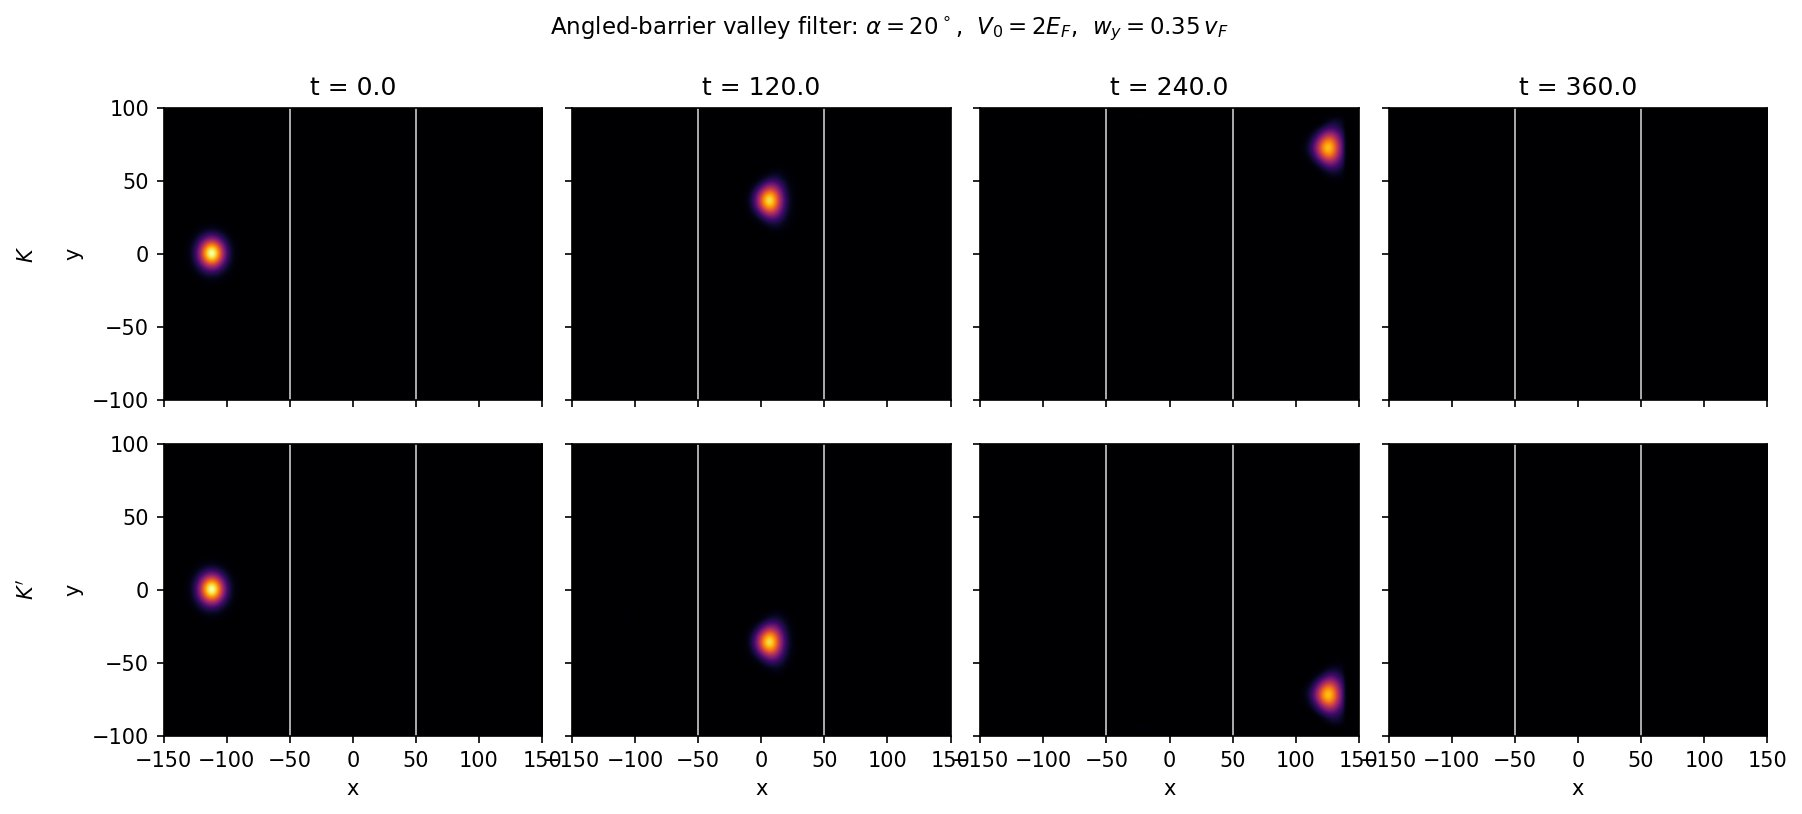
\includegraphics[width=0.9\textwidth]{figs/fig_ex1_rect.png}
\caption{Example~1 control: rectangular barrier ($\alpha=0$) at
         $V_0=1.75\,\EF$, $w_y=0.3\,\vF$. The $K$ (top) and
         $K^\prime$ (bottom) wave packets evolve as mirror images
         about $y=0$ and transmit with identical integrated weight
         ($T_K=T_{K^\prime}=0.976$, $\eta=0$). The tilt produces
         transverse separation but not net polarisation.}
\label{fig:ex1_rect}
\end{figure*}

\begin{figure*}[t]
\centering
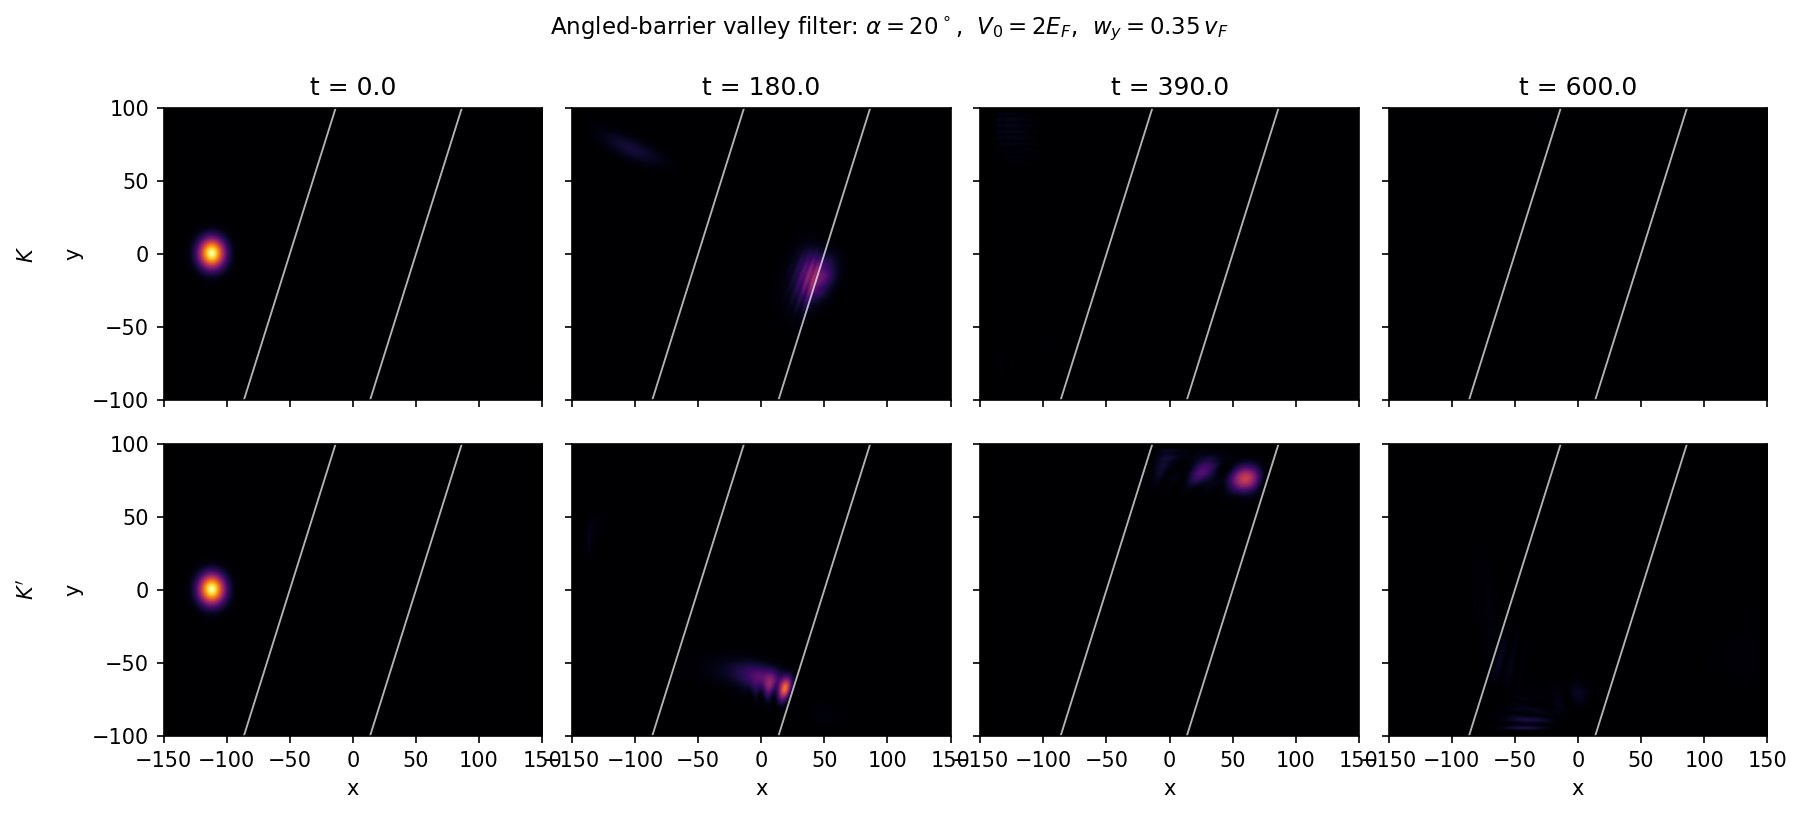
\includegraphics[width=0.9\textwidth]{figs/fig_ex1_angled.png}
\caption{Example~1 filter: angled barrier ($\alpha=20^\circ$) at
         $V_0=1.75\,\EF$, $w_y=0.3\,\vF$. The $K$ wave packet (top)
         transmits cleanly through the rotated gate to the right
         drain, while the $K^\prime$ packet (bottom) hits the
         interface at unfavourable angles and is largely reflected,
         producing $\eta=+0.265$.}
\label{fig:ex1_angled}
\end{figure*}

\begin{figure}[h]
\centering
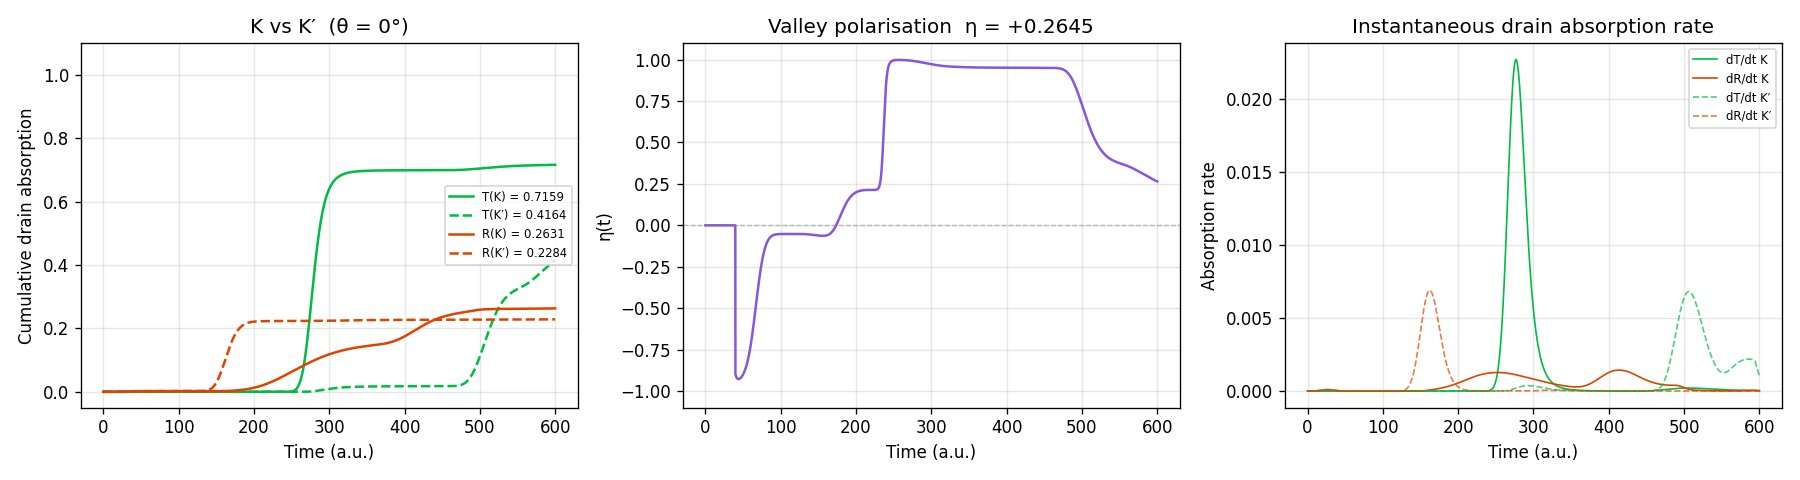
\includegraphics[width=\linewidth]{figs/fig_ex1_transport.png}
\caption{Cumulative drain absorption, transient valley polarisation
         $\eta(t)$, and instantaneous absorption rate for the
         angled barrier run. The $K^\prime$ reflected component
         reaches the source drain ($R$) before the $K$ transmitted
         component reaches the drain ($T$), driving $\eta(t)$
         through strongly non-monotonic transient values before
         settling to the asymptotic $\eta=+0.265$.}
\label{fig:ex1_transport}
\end{figure}

\subsection{Example 2: angular dependence of Klein tunneling}
\label{sec:ex2}

The second example scans the injection angle through a rectangular
barrier in an untilted isotropic channel, with $V_0=2\,\EF$
(deep bipolar Klein regime) and barrier width $d\approx100$ in sim
units. A single-valley run is sufficient because at zero tilt $K$ and
$K^\prime$ are equivalent. Four angles
$\theta\in\{-15^\circ,-5^\circ,+5^\circ,+15^\circ\}$ are swept in a
loop within a single script invocation, and the resulting
transmission and reflection are tabulated together with the mirror
symmetry residuals (Table~\ref{tab:ex2}).

\begin{table}[ht]
\centering
\caption{Example 2 results. Mirror-symmetry residuals
$|\Delta T|=|T(+\theta)-T(-\theta)|$ are at the single-precision level.}
\label{tab:ex2}
\begin{tabular}{rcccc}
\hline
$\theta$ (deg) & $T$ & $R$ & $T+R$ & $|\Delta T|$ \\
\hline
$-15$ & 0.868 & 0.126 & 0.994 & --- \\
$-5$  & 0.974 & 0.021 & 0.995 & --- \\
$+5$  & 0.974 & 0.021 & 0.995 & $4\times10^{-6}$ \\
$+15$ & 0.868 & 0.126 & 0.994 & $1\times10^{-6}$ \\
\hline
\end{tabular}
\end{table}

The transmission profile has the expected Klein character: $T$ is
close to unity near $\theta=0$ and drops off with $|\theta|$. The
mirror-symmetry residuals between the $\pm5^\circ$ and $\pm15^\circ$
pairs agree to the $10^{-6}$ level, confirming the propagator's
numerical symmetry. A single oblique-injection run also displays the
Veselago-type negative refraction at the $p$--$n$ interfaces: the
transmitted beam emerges on the opposite transverse side relative
to what a same-sign refraction would predict, reproducing in wave
packet form the trajectory bending predicted by Dirac-fermion
electron optics \cite{Cheianov2007,Nguyen2018}. Figure~\ref{fig:ex2_snapshots}
shows the four-angle snapshot grid and Fig.~\ref{fig:ex2_summary}
the $T(\theta)$ and $R(\theta)$ summary.

\begin{figure*}[t]
\centering
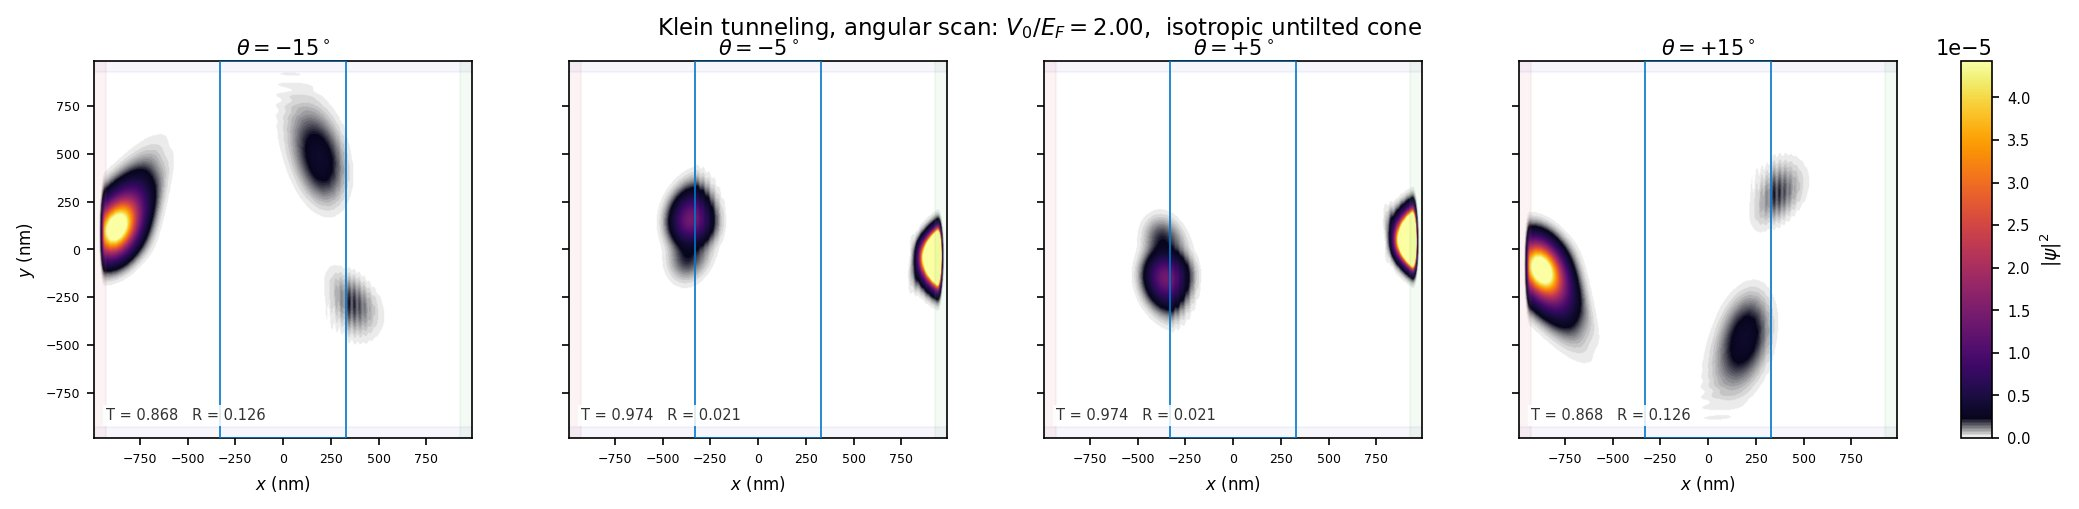
\includegraphics[width=0.95\textwidth]{figs/fig_ex2_snapshots.png}
\caption{Example~2 snapshot grid for the four-angle Klein scan.
         Each panel is a late-time snapshot at the indicated
         injection angle through a rectangular barrier at
         $V_0=2\,\EF$; the single-valley run is sufficient because
         at zero tilt $K\equiv K^\prime$. The mirror symmetry
         between $\pm\theta$ panels is exact to single-precision
         (Table~\ref{tab:ex2}).}
\label{fig:ex2_snapshots}
\end{figure*}

\begin{figure}[h]
\centering
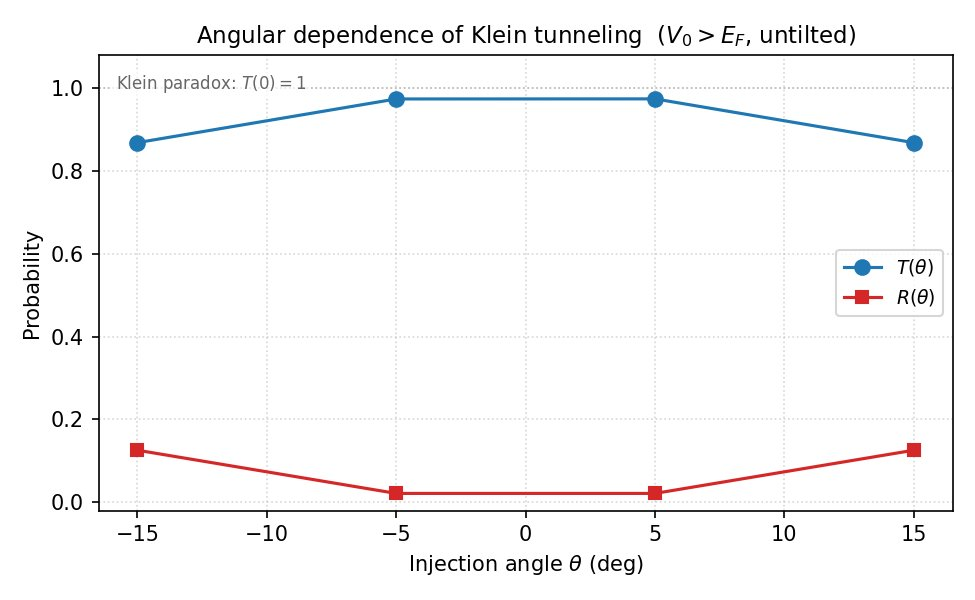
\includegraphics[width=\linewidth]{figs/fig_ex2_summary.png}
\caption{Angular dependence of Klein tunnelling, $V_0=2\,\EF$,
         untilted isotropic cone. $T(\theta)$ (blue) approaches the
         Klein-paradox value $T=1$ at $\theta=0$ and decreases with
         $|\theta|$; $R(\theta)$ (red) is the complement. The
         $\pm\theta$ pairs are numerically coincident.}
\label{fig:ex2_summary}
\end{figure}

% =======================================================================
\section{Performance}
\label{sec:performance}
% =======================================================================

A single production run at the worked-example resolution
($512^2$ grid, $1.5\times10^4$ time steps, dual-valley) completes in
roughly 10--30 minutes on a modern 8-core CPU with pyFFTW installed,
or on a single mid-range GPU. Memory use is dominated by
single-precision spinor storage and scales as
$N_x N_y \times 16\,\text{B}\times N_\mathrm{copies}$; a $512^2$
dual-valley run requires ${\sim}1$\,GB of RAM. The parallel sweep
driver distributes $V_0$ tasks across workers with near-linear
scaling up to approximately one worker per physical core; fine-grained
FFT threading tends to under-perform single-threaded FFT workers at
fixed core count in this problem size regime. State checkpoints are
kept small (${\sim}1$\,kB per task) so that interrupted sweeps can be
resumed without loss of progress.

% =======================================================================
\section{Discussion and outlook}
\label{sec:discussion}
% =======================================================================

\dirac covers the continuum-Dirac transport regime for 2D systems
with tilted and anisotropic cones; it is not a replacement for
tight-binding scattering-matrix codes such as \textsc{Kwant}
\cite{Groth2014}, which remain the appropriate tool for lattice
problems and for stationary transport in multi-terminal geometries.
Within its scope, several limitations follow from design choices.
The numerical grid is uniform Cartesian, which is inefficient for
devices with strongly multi-scale features; adaptive meshing is not
currently supported. The intervalley coupling is modelled as a
spatially local, pseudospin-preserving scalar, which captures
barrier-mediated and line-defect physics but not phonon-assisted or
long-range spin--orbit-mediated intervalley scattering. Magnetic
fields and spin--orbit coupling are not included in this release.
All computations are performed in single precision; double-precision
support is straightforward to add but has not been a priority.

Planned extensions include (i) a companion package for
valley-resolved phase extraction from saved wavefunction snapshots,
which underlies a separate manuscript on electrostatic valley phase
gates in tilted Dirac channels; (ii) GPU acceleration via CuPy, for
which the split-operator structure maps naturally; and (iii) a minor
upgrade of the coupled propagator to non-local intervalley kernels
$U_{KK^\prime}(\mathbf{k})$. Pull requests and bug reports are welcome
through the repository.

% =======================================================================
\section*{Acknowledgments}
% =======================================================================

The author thanks the Nanoelectronics Research Center (Nano
Electronics Research M\"uhendislik Ar. Ge. Ltd. \c{S}ti., Istanbul)
for computational resources. A.\,D.\,Zabolotskii is thanked for
helpful correspondence on the 8-Pmmn borophene tight-binding model.

% =======================================================================
\section*{Code availability}
% =======================================================================

\dirac v1.0 is available at
\href{https://github.com/can-yesilyurt/Dirac-Wavepacket}{github.com/can-yesilyurt/Dirac-Wavepacket}
and is archived as a CPC Library entry (identifier to be assigned).
The version used in this manuscript corresponds to the v1.0 release.

% =======================================================================
\begin{thebibliography}{99}

\bibitem{CastroNeto2009}
A.\,H. Castro Neto, F. Guinea, N.\,M.\,R. Peres, K.\,S. Novoselov,
A.\,K. Geim, Rev.\ Mod.\ Phys.\ \textbf{81} (2009) 109.

\bibitem{Goerbig2008}
M.\,O. Goerbig, J.-N. Fuchs, G. Montambaux, F. Pi\'echon, Phys.\ Rev.\
B \textbf{78} (2008) 045415.

\bibitem{Kong2021}
Z. Kong, J. Li, Y. Zhang, S.-H. Zhang, J.-J. Zhu,
Nanomaterials \textbf{11} (2021) 1462.

\bibitem{Zhang2018}
S.-H. Zhang, W. Yang, Phys.\ Rev.\ B \textbf{97} (2018) 235440.

\bibitem{Nguyen2018}
V.\,H. Nguyen, J.-C. Charlier, Phys.\ Rev.\ B \textbf{97} (2018)
235113.

\bibitem{LopezBezanilla2016}
A. Lopez-Bezanilla, P.\,B. Littlewood, Phys.\ Rev.\ B \textbf{93}
(2016) 241405(R).

\bibitem{Zabolotskiy2016}
A.\,D. Zabolotskiy, Y.\,E. Lozovik, Phys.\ Rev.\ B \textbf{94}
(2016) 165403.

\bibitem{Soluyanov2015}
A.\,A. Soluyanov, D. Gresch, Z. Wang, Q. Wu, M. Troyer, X. Dai,
B.\,A. Bernevig, Nature \textbf{527} (2015) 495.

\bibitem{Wang2019}
Q. Wang, C. Yesilyurt, F. Liu, Z.\,B. Siu, K. Cai, D. Kumar, Z. Liu,
M.\,B.\,A. Jalil, H. Yang, Nano Lett.\ \textbf{19} (2019) 2647.

\bibitem{Pereira2009}
V.\,M. Pereira, A.\,H. Castro Neto, Phys.\ Rev.\ Lett.\ \textbf{103}
(2009) 046801.

\bibitem{Oliva2020}
M. Oliva-Leyva, G.\,G. Naumis (2020), various refs (placeholder).

\bibitem{Cheianov2007}
V.\,V. Cheianov, V. Fal'ko, B.\,L. Altshuler, Science \textbf{315}
(2007) 1252.

\bibitem{Katsnelson2006}
M.\,I. Katsnelson, K.\,S. Novoselov, A.\,K. Geim, Nat.\ Phys.\
\textbf{2} (2006) 620.

\bibitem{Berry1987}
M.\,V. Berry, R.\,J. Mondragon, Proc.\ R.\ Soc.\ A \textbf{412}
(1987) 53.

\bibitem{Groth2014}
C.\,W. Groth, M. Wimmer, A.\,R. Akhmerov, X. Waintal, New J.\ Phys.\
\textbf{16} (2014) 063065.

\bibitem{Kloss2021}
T. Kloss, J. Weston, B. Gaury, B. Rossignol, C. Groth, X. Waintal,
New J.\ Phys.\ \textbf{23} (2021) 023025.

\bibitem{Mocken2008}
G.\,R. Mocken, C.\,H. Keitel, Comput.\ Phys.\ Commun.\ \textbf{178}
(2008) 868.

\bibitem{Schmidt2019}
B. Schmidt, U. Lorenz, Comput.\ Phys.\ Commun.\ \textbf{228} (2018)
197.

\bibitem{Chaves2015}
A. Chaves, G.\,A. Farias, F.\,M. Peeters, R. Ferreira,
Commun.\ Comput.\ Phys.\ \textbf{17} (2015) 850.

\end{thebibliography}

\end{document}
